\chapter{Search with Non-Resonance Signatures (Vector Boson Scattering)}
\chapterquote{When something is too hard, there is always another way.}{Charlie, Finding Dory}

In addition to the physics with resonance particles, unknown couplings between SM particles are also a portal to new physics. Their signature would be similar to SM with enhanced or reduced (interference) occurrence rates (cross section) for the physical process of interest. However, the deviation from SM prediction would be marginal, so tests on precision measurement could only be achieved with large amounts of data. 
\\
\\This analysis is aiming for the phenomenology with ``vector boson scattering'' (VBS) which has the signature like VBF with one back-to-back high-mass jet pair accompanied by two SM gauge bosons ($qq \to VVqq$). The phenomenon was predicted by SM and measured in ATLAS Run1 data analysis (2009-2012) with the search for the anomalous quadratic gauge coupling (aQGC), but it didn't give a promising result\cite{STDM-2014-05} for the existence. This analysis is to extend the search with greater luminosity of data collected in 2015 and 2016 for $36.1fb^{-1}$, and the final state of the dibson system is chosen to be semileptonic. This analysis will focus on one lepton channel ($WV \to l\nu qq$) just like the the resonance search, and the result will be combined with other two semileptonical final states ($ZV \to \nu\nu qq/llqq$) for the statistic interpretation.
\\
\\With the same final state, the object definition was inherited from the resonance search, and the simulation sample and dataset are also reused. However, because the search is aiming for different signal, the optimization was repeated for the thresholds of object and event selection.  The most significant change in this analysis is that although $m_{WV}$ is still reconstructed, it cannot be taken as the discriminant because of no resonance particle in the process. Instead, an algorithm of boosted decision tree (BDT) is performed on the physical object observables, and it would give the output of ``BDT score'' for the discrimination of signal and background.
\\ 
\\To maximize the sensitivity, the event categorization employs the same strategy to have boosted HP, boosted LP, and resolved regions for signal, W+jet and $t\bar{t}$ control regions for VBS category only, and the event priority is the same as the resonance search.
\section{Signal Simulation Samples}
Two types of signal signature were generated: SM VBS scattering and anomalous quadratic coupling. As this analysis is a general search for the coupling signature, a couple of physical physical processes are involved as the signal. In this case, an approximation of effective field theory (EFT) is applied to simplify the simulation. 

\subsection{Standard Model Vector Boson Scattering}
Under the SM, the vector boson scattering is through the coupling to a variety of bosons including W/Z bosons, photon, or Higgs boson. The coupling strength is constrained by the Higgs mass, so the measurement could be another test on the Higgs naturalness and  Brout-Englert-Higgs Mechanism\cite{PhysRevD.7.3111}. The interactions considered in this analysis are shown in Fig. \ref{Fig:feynmanVBS}  with the order of $\alpha_{EW}^6$ which also considers the decays of bosons into fermions. 

\begin{figure}[tbp]
	\begin{center}
		\subfloat[]{
			\includegraphics[width=0.3\textwidth,keepaspectratio]{Chapter5/feynVBS2.pdf}
		}
		\subfloat[]{
			\includegraphics[width=0.3\textwidth,keepaspectratio]{Chapter5/feynVBS3.pdf}
		}\\
		\subfloat[]{
			\includegraphics[width=0.3\textwidth,keepaspectratio]{Chapter5/feynVBS4.pdf}
		}
		\subfloat[]{
        	\includegraphics[width=0.3\textwidth,keepaspectratio]{Chapter5/feynVBS1.pdf}
        }
		\subfloat[]{
			\includegraphics[width=0.3\textwidth,keepaspectratio]{Chapter5/feynVBS5.pdf}
		}
		\caption{
			Here are the Feynman diagrams which contribute to the SM VBS signal. The dashed line in figure (b) and (d) are the Higgs boson which couples the interactions. Those interactions are of the order $\alpha_{EW}^6$ involving the consideration of the decays of the two scattered bosons into fermions. 
		}
		\label{Fig:feynmanVBS}
	\end{center}
\end{figure} 

\noindent
For those interactions, only the longitudinal component of bosons is considered, while the transverse one has relatively low coupling strength, so it is neglected\cite{Brass:2018hfw}. When the Higgs boson is not involved in the interactions (Fig. \ref{Fig:feynmanVBS} (a)-(c)), the coupling magnitude\cite{Barger:1990py} could be presented in Mandelstam variables as:
\begin{equation}
|\mathcal{M}|=\frac{g^2}{4m_{W}^{2}}\left[s+t\right]
\end{equation}
with the consideration of only the coupling to W bosons for simplicity. This implies that the coupling strength will diverge when the energy increases, so the unitary of $\rho$ in Eq. \ref{Eq:rho} would be broken due to the enhanced coupling between W and Z bosons. The introduction of the Higgs boson to mediate the bosons could provide a constraint to prevent the divergence, which makes the coupling magnitude to:
\begin{equation}
|\mathcal{M}|=\frac{g^2m_{H}^2}{4m_{W}^{2}}\left[\frac{t}{t-m_{H}^{2}}+\frac{s}{s-m_{H}^{2}}\right]
\end{equation} 
This expression is hold at the tree level, and the perturbative terms are neglected with the light Higgs boson\cite{Rindani:2009gm}. However, the high order terms would remain if the Higgs mass is above $1.2TeV$ with $\lambda > 4\pi$:
\begin{equation}
m^2_{H}=2\lambda\nu^2 > 1.2TeV
\end{equation}
where $\nu$ is $246GeV$ measured from the experiments. This would then make the cross-section diverge again as shown in Fig. \ref{Fig:VBSXS_heavyhiggs}. Therefore, the cross-section measurement of the SM vector boson scattering could be another verification of the existence of high-mass Higgs boson.  

\begin{figure}[tbp]
	\begin{center}
		\includegraphics[width=0.8\textwidth,keepaspectratio]{Chapter5/VBSXS_heavyhiggs.png}
		\caption{The cross-section of vector boson scattering between gauge bosons with Higgs boson of $125GeV$ and $10^{10}GeV$ as a function of $\sqrt{s}$.\cite{Schnoor:2000941}}
		\label{Fig:VBSXS_heavyhiggs}
	\end{center}
\end{figure} 
\noindent
{\bf Sample Production}
\\
\\The signal samples are produced with the setting under SM with Higgs boson mass at $125GeV$. \textsc{MADGRAPH5\_aMC@NLO v2.3.3}\cite{Alwall:2014hca} is the chosen generator interfaced by \textsc{PYTHIA8}\cite{Sjostrand:2007gs} for the fragmentation with the PDF set of \textsc{NNPDF30LO}\cite{Ball:2012cx}. The two medium state bosons are required to be on-shell with the mass pole from PDG. 
\\
\\As the generation command in the generator is $pp \to VVjj$, so some of the unwanted interaction would also go into the signal samples. Their coupling is still at the order of $\alpha_{EW}^6$, but no VBS interaction is involved. With the VBS requirement on event selection, the contribution is well-suppressed. 
\noindent
\subsection{Anomalous Quadratic Coupling (aQGC)}
With the light mass of the discovered SM Higgs boson, the Higgs naturalness turns to be an problem. In addition to the BSM heavy Higgs bosons, the hidden couplings between bosons is another approach to this issue. It could lead to the fine-tuning to the SM Lagrange to make high order correction. 
\\
\\To simplify the hidden theory, the approach of EFT is applied which could be presented in Lagrange as:
\begin{equation}
\mathcal{L}_{EFT} = \mathcal{L}_{SM} + \sum_{i}\frac{\mathcal{C}_i}{\Lambda_{i}^{d-4}}\mathcal{O}^{d}_{i}
\end{equation}
where the extended term, $\sum_{i}\frac{\mathcal{C}_i}{\Lambda_{i}^{d-4}}\mathcal{O}^{d}_{i}$, is contributed from the anomalous couplings. It is constructed by 3 components: $\Lambda$ as the energy scale for where the coupling is significant, $C_{i}$ as the coefficient of this interaction and $O^{d}_i$ is the operator. $d$ is used as the number of dimensions of this coupling. With the constraint of $\Lambda$ in the power of $d-4$\footnote{$d-4$ is applied on the energy scale to keep the dimension consistent in the Lagrangian}, the interactions of higher order could be neglected due to small contribution. When $\Lambda$ goes to $\infty$, that would mean the new physics is unapproachable, and SM would be the only observable phenomenon. This approach has been proven working well to have theoretical agreement to experimental data with the example from Fermi theory. 
\\
\\The new physics operators, $\mathcal{O}$, considered here is based on Eboli model\cite{Eboli:2016kko,Eboli:2000ad} which formulates the new interactions with the components:
\begin{itemize}
	\item{Higgs Field Covariant Derivative}: $D_{\mu}\Phi =(\partial_\mu + igW^j_{\mu}\frac{\sigma^{j}}{2}+ig'B_\mu\frac{1}{2})\Phi $
	\item{Electroweak W Field Covariant Derivative}: $\hat{W}_{\mu\nu}=\sum_{i}(\partial_\mu W_\nu^i - \partial_\nu W_\mu^i)\frac{\sigma^i}{2}$
	\item{Electroweak B Field Covariant Derivative}: $B_{\mu\nu} = \partial_\mu B_\nu - \partial_\nu B_\mu$
\end{itemize}
The notations used here are the same as the ones used in Chpater 1 with $\sigma^j$ as the Pauli Matrix, and they all have the same dimension of two:
\begin{equation}
\left[D_{\mu}\Phi\right]=\left[\hat{W}_{\mu\nu}\right]=\left[B_{\mu\nu}\right]= GeV^2
\end{equation}
Then, the BSM interaction is constructed from four of them (the same component could be chosen multiple times) which are combined into one individual operator with the dimension of eight. three types of operators can then be categorized by the combinations:
\begin{itemize}
    \item{$D_\mu\Phi$ only}: the operators are only composed of $D_\mu\Phi$ and denoted as $\mathcal{O}^i_S$ with the free parameters $f^i_{S}$. The index ranges from 0 to 2.  
    \item{all the elements}: the operators are the mix with all the components denoted as  $\mathcal{O}^i_M$. The free parameters are denoted as $f^i_{M}$ with the index ranging from 0 to 7.
    \item{combination of the electroweak fields}: the operators have $\hat{W}_{\mu\nu}$ and $B_{\mu\nu}$ which are denoted as $\mathcal{O}_{T}^i$ with the free parameters, $f_T^i$. The index has the range from 0 to 9. 
\end{itemize}
\noindent
\\
\\{\bf Signal Production}
\\
\\It is impossible to investigate all the possible operators, so only one operator of each category is chosen in the signal, which are $O_{S}^0$, $O_{M}^0$, and $O_{T}^0$ with the free parameter, $f^0_{S}$, $f^0_{M}$,  $f_T^0$, while the other operators are tuned to 0.  The chosen coupling strength for the free parameters in the simulation is summarized in Tab. \ref{Tab:Eboli}.
\\
\\Similar to the SM VBS signal, the production is also via \textsc{MADGRAPH5\_aMC@NLO v2.3.3}\cite{Alwall:2014hca} interfaced by \textsc{PYTHIA8}\cite{Sjostrand:2007gs} with the PDF set of NNPDF30LO\cite{Ball:2012cx}. 
\begin{table}[h]
	\caption{Set-up of parameters in Eboli Model for this analysis} \label{Tab:Eboli}
	\begin{center}
		\begin{tabular}{ | c | c | c | c | }
		\hline
			     &   $f^0_{S}\left[10^{-12}TeV\right]$  & $f^0_{M}\left[10^{-12}TeV\right]$ & $f^0_{T}\left[10^{-12}TeV\right]$ \\
	    \hline
	    Signal 1 &        50                            & 0                                & 0 \\
	    \hline
		Signal 2 &        0                             & 5                                & 0 \\
		\hline
		Signal 3 &        0                             & 0                                & 1 \\
		\hline
		\end{tabular}
	\end{center}
\end{table}
\noindent
\subsection{Interference Effect on the Signal}
The simulation on the signal and backgrounds are done respectively, so the interference effect is not taken into account for the cross-section estimation. Under the Standard Model, the interference on the VBS cross-section would come from the QCD processes which is via the same process, $qq\to VVjj$, under the order of coupling, $\alpha_{EW}^4\alpha_{EW}^2$. The QCD interactions could be seen in Fig.~\ref{Fig:feynmanQCD}.
\begin{figure}[tbp]
	\begin{center}
		\subfloat[]{
			\includegraphics[width=0.3\textwidth,keepaspectratio]{Chapter5/feynQCD2.pdf}
		}
		\subfloat[]{
			\includegraphics[width=0.3\textwidth,keepaspectratio]{Chapter5/feynQCD3.pdf}
		}\\
		\subfloat[]{
			\includegraphics[width=0.3\textwidth,keepaspectratio]{Chapter5/feynQCD4.pdf}
		}
		\subfloat[]{
			\includegraphics[width=0.3\textwidth,keepaspectratio]{Chapter5/feynQCD1.pdf}
		}
		\subfloat[]{
			\includegraphics[width=0.3\textwidth,keepaspectratio]{Chapter5/feynQCD5.pdf}
		}
		\caption{
			Here are the Feynman diagrams which contribute to the SM VBS signal. The dashed line in figure (b) and (d) are the Higgs boson which couples the interactions. Those interactions are of the order $\alpha_{EW}^6$ involving the consideration of the decays of the two scattered bosons into fermions. 
		}
		\label{Fig:feynmanQCD}
	\end{center}
\end{figure}
The effect on the cross-section estimation could be presented with the matrix elements, $\mathcal{M}$: 
\begin{equation}
|\mathcal{M}|^2=|\mathcal{M}_1+\mathcal{M}_2|^2 = |\mathcal{M}_1|^2+|\mathcal{M}_2|^2+2Re(\mathcal{M}_1\mathcal{M}_2)
\end{equation}
with $|\mathcal{M}|^2$ as the total amplitude, and $\mathcal{M}_1$ and $\mathcal{M}_2$ are the amplitudes from the VBS and QCD contributions. The last term is showing the interference effect on the total cross-section. With the estimation by \textsc{MadGraph5\_aMC@NLO v2.3.3}\cite{Alwall:2014hca}, this effect is less around $1\%$ for the VBS signal, so it is taken negligible, but it is still taken as one contribution of systematic uncertainty.
\section{Event Selection}
In general, the event selection in this analysis has the same scheme as the resonance search including both trigger and event cleaning. However, as the optimization is conducted with SM VBS signal, some cuts are looser due to the similar kinematic properties with respect to the background. For the same reason, the cuts on topological variables employed in resonance search would also remove significant signal, so they are dropped in this analysis.
\\
\\Not just the event selection scheme but also the event categorization is adopted here from the resonance $WV\to \ell\nu qq$ analysis. Three regions are defined with the jet topology as boosted HP, boosted LP, resolved regions (in the order of selection priority) for W+jet control region, top control region, and signal regions (with higher selection priority than the other two). To achieve better sensitivity for aQGC, the dedicated control region is defined with one addition cut in the siganl region with $m^{VBS}_{jj}>1TeV$. 
\subsection{Batman Veto}
In September 2017, a cell saturation problem in high pile-up runs in 2015 and 2016 was reported in the LAr detector endcap (EMEC). This leads to a large number of low $p_{T}$ jets ($p_{T}>20~GeV$) falsely reconstructed at $|\eta|\sim 2.9$ (which is beyond the range where jvt is applicable), and they also made the contribution to $E^{miss}_{T}$ reconstruction. Therefore, the events are removed manually by the event and run numbers. Fig. \ref{Fig:batman_veto} shows the jet $\eta$ distributions before and after the problematic event removal in resolved signal region but with 2 loose lepton selected which is another channel along with this 1 lepton analysis. 
\begin{figure}[tbp]
	\begin{center}
		\includegraphics[width=0.8\textwidth,keepaspectratio]{Chapter5/SR_EtaTagResJet_BatmanVeto}
		\caption{The jet $\eta$ distribution before (left) and after (right) the problematic event removal}
		\label{Fig:batman_veto}
	\end{center}
\end{figure} 
 
\subsection{VBS Event Selection}
The pair of VBS jets are still chosen to be the one with the highest invariant mass and toward different $\eta$ direction ($\eta_1\times\eta_2<0$) in a event, but, different to resonance search, the selection shall be conducted after the pair of signal jets from the boson decay (the pair with invariant mass most close to W/Z mass pole) to achieve better sensitivity in resolved region. The full selection of the jet pair is listed below:
\begin{itemize}
	\item $p_{T}^{j1}>30GeV\&\&p_{T}^{j2}>30GeV$
	\item $m_jj^{VBS}>400GeV$
	\item $\eta_1\eta_2<0$
	\item no b-tagged
\end{itemize}
\subsection{Boosted $\&$ Resolved Event Selection}
Tab. \ref{tab:SRdefinitionsVBS} and \ref{Tab:SRdefinitions_resolvedVBS} are showing the cuts applied to select the events into both signal and control regions. The measurement on both aQGC and SM cross-section doesn't distinguish the processes of WW or WZ, so only one SR is defined for both boosted and resolved jet topologies.
\\
\\As compared to the resonance search, object selections are kept the same like the $p_{T}$ threshold or lepton isolation requirements. However, the $E^{T}_{miss}$ cut is lowered to $80GeV$ to enhance the statistics for the training sample into the multivariable analysis. Furthermore, the topological cuts are also removed from this analysis, because they are too stringent for the signal sample. And, the b-tagging requirement is also changed in the resolved channel with forbidding any b-tagged jet in the events for signal region. 
\\
\\The definition of W+jet control regions is still defined by the mass side band of the dijet system in resolved channel and failed mass tagging in boosted channel. With the change on number of b-tagged jets, the top control region definition is also simplified as the event with any existence of b-jets.  
\begin{table}[t]
	\caption{Summary of the selection criteria in the definition of the signal region (SR), $W$+jets control region ($W$ CR) and $t\bar{t}$ control region ($t\bar{t}$ CR), in the high-purity (HP) and low-purity (LP) categories.  } \label{tab:SRdefinitionsVBS}
	\begin{center}
		\begin{adjustbox}{center}
			\begin{tabular}{|l|l|c|c|c|c|c|c|}
				\hline
				\multicolumn{2}{|l|}{\multirow{2}{*}{Selection}} & \multicolumn{2}{c|}{SR}  &  \multicolumn{2}{c|}{$W$ CR}  & \multicolumn{2}{c|}{$t\bar{t}$ CR} \\
				\cline{3-8}
				\multicolumn{2}{|l|}{} & HP & LP &HP & LP & HP & LP \\
				\hline
				\multirow{3}{*}{$W\rightarrow l\nu$} & Num of signal leptons & \multicolumn{6}{c|}{ 1 } \\
				\cline{2-8}
				&Num of vetoed leptons & \multicolumn{6}{c|}{ 0 }  \\
				\cline{2-8}
				&\vphantom{\Large B} $E^{miss}_{T}$ & \multicolumn{6}{c|}{ $>80GeV$ } \\
				\hline
				\multirow{5}{*}{$W/Z\rightarrow J$} & Num of large-$R$ jets & \multicolumn{6}{c|}{ $\geq 1$ } \\
				\cline{2-8}
				& \vphantom{\Large B} $D^{(\beta=1)}_2$ 50\,\% WP & pass & fail & pass & fail & pass & fail \\
				\cline{2-8}
				& \vphantom{\Large B} $D^{(\beta=1)}_2$ 80\,\% WP & --- & pass  & --- & pass  & --- & pass \\
				\cline{2-8}
				& $W/Z$ mass 50\,\% WP & pass &fail& --- & --- & pass & fail\\
				\cline{2-8}
				& $W/Z$ mass 80\,\% WP &  --- & pass & fail & fail & --- & pass\\
				\hline
				Top-quark veto & Num of $b$-tagged jets & \multicolumn{4}{c|}{0} & \multicolumn{2}{c|} {$\geq 1$} \\
				\hline
			\end{tabular}
		\end{adjustbox}
	\end{center}
\end{table}
\begin{table}[t]
	\caption{Summary of the selection criteria of of the  the resolved analysis for the $WW$ and $WZ$ signal regions (SR), $W$+jets control region (WR) and $ t\bar{t}$ control region (TR). } \label{Tab:SRdefinitions_resolvedVBS}
	\begin{center}
		\resizebox{\textwidth}{!}{
			\begin{tabular}{|l|l|c|c|c|}
				\hline
				\multicolumn{2}{|l|}{cuts} & SR & WR & TR \\
				\hline
				\multirow{3}{*}{$W\rightarrow \ell\nu$ selection} & Number of signal leptons & \multicolumn{3}{c|}{ 1 } \\
				\cline{2-5}
			  	                                                  &Number of veto leptons    & \multicolumn{3}{c|}{ 0 }  \\
				\cline{2-5}
				                                                  &$E^{miss}_{T}$ & \multicolumn{3}{c|}{ $>80GeV$ } \\
				\hline
				\multirow{4}{*}{$W/Z\rightarrow jj$ selection}    & Number of small jets & \multicolumn{3}{c|}{ $\geq2$ } \\ 
				\cline{2-5}
			                                                    	& $\pt (j1)$ & \multicolumn{3}{c|}{ $>60$~GeV}\\
				\cline{2-5}
				                                                  & $\pt (j2)$ & \multicolumn{3}{c|}{ $>45$~GeV}\\
				\cline{2-5}
				                                                  & $m_{jj}$ & [64, 106]GeV\ & $<66GeV$         &  [64, 106]GeV \\
			                                                    	&          &               & or [106, 200]GeV & \\
				\hline
				Top veto & Number of $b$-tagged jets& 0 & 0 & $ \geq1$ \\
				\hline
				\multicolumn{2}{|c|}{Existence of VBF jets} & \multicolumn{3}{c|}{yes} \\
				\hline
			\end{tabular}
		}
	\end{center}
\end{table}
\section{Multivariate Analysis}
When the new physics and SM interactions have similar kinematics, their detector signatures would have marginal difference. In this case, no individual variable could be taken as the discriminant to distinguish signal from backgrounds. And, this is why the multivariate analysis is taken into the analysis, and it is based on the framework of TMVA\cite{Hocker:2007ht}.
\\
\\Two candidate algorithms were considered: adaptive and gradient decision tree. However, the outcome of adaptive decision tree is not robust to prevent overtraining. This means the outcome might only have the distinguishing power to the training sample, but the appliance outside is less powerful. Therefore, gradient boost decision (GBDT) is chosen to be used in this analysis.
\\
\\{\bf Decision Tree}
\\
\\Decision tree is constructed with a series of binary decisions. Those decisions are made by whether the events could pass ``a'' cut which can give the best prediction. Two types of decision tree are defined by  signal and background separation. The full scheme could be presented as Fig. \ref{Fig:decision_tree}.
\begin{figure}[tbp]
	\begin{center}
		\includegraphics[width=0.7\textwidth,keepaspectratio]{Chapter5/DT.png}
		\caption{The scheme of a decision tree. The nodes are where the decision are made by whether the event could pass the cut on $x_i$, $x_j$, and $x_k$. The bottom nodes are the final outcomes labeled as S for more signal events categorized into the node, and B for more background events}
		\label{Fig:decision_tree}
	\end{center}
\end{figure} 
To make the best decision on signal and background separation, the \textit{Gini Index} is defined as:
\begin{equation}
I_{G}= p(1-p)
\end{equation}
where p is the percentage of signal events (purity) in the node. The decision would then be made to optimize the increase of $I_{G}$ in the mother node:
\begin{equation}
Gain = I_{G}^{\text{mother}}-\frac{n_{1}}{N}I_{G}^{\text{daughter1}}-\frac{n_{2}}{N}I_{G}^{\text{daughter2}}
\end{equation} 
where the two daughter nodes are split from the mother node (event number, $N$, divided to $n_{1}$ and $n_{2}$), and their $I_{G}$'s are reweighted. After repeating this procedure, the events get into the leaf nodes where they are label by signal or background depending on which kind of events takes over bigger proportion. To avoid over-training, a further procedure called ``prunning'' is applied. This procedure is conducted from the bottom, and the node with little increase of the separation power (\textit{Gini Index}) is removed. If the following branches are all removed, the mother node making the decision would be turned into another leaf node. 
\\
\\The other decision tree is also used in this analysis which is called ``regression tree'' for the prediction of a truth value which is not in the binary format. In this case, the \textit{Gini Index} is not available, and, instead, the average squared error is used:
\begin{equation}
\sigma = \frac{1}{N}\sum^{N}(\hat{y}_i-y^{truth}_i)
\end{equation}
with $\hat{y}_i$ as the average truth value of the events in the same node and $y^{truth}_i$ as the truth value of the events itself. The decision is made with a cut which makes $\sigma$ as the minimum.
  
In general, Decision tree has the advantage of being handy for use, easy to understand, and flexible, but it also has the disadvantage of being weak to statistic fluctuation and correlation between input variables especially when only one tree is trained. Therefore, there are a couple of methods to train trees into ``forests'' like random forest, and the one used in this analysis is ``Gradient Boost''.
\\
\\{\bf Gradient Boost}
\\
\\Due to the insufficiency of decision tree, the approach called ``boost'' is applied into the sample events after each tree is grown up. The process is determined by deviation of the predicted value from the truth value with a ``Loss Function'' defined as:
\begin{equation}
L(F(x_{i}), y_{i}) = \sum_{i}^{n}\ln(1+\exp{(-2F(x_i)y_{i})})
\end{equation} 
where $F(x_{i})$ is the predicted value from the outcome of decision trees for the $i$th event, and $y_{i}$ is its truth value. The training process is then conducted in the following steps:
\begin{enumerate}[(a)]
	\item  The first tree is built up with the procedure as mentioned above to optimize the \textit{Gini Index}.
	\item  The predicted value of each event, $F_{0}(x_i)$, is then assigned by the type of nodes. (signal node: $F_{0}(x_i)=1$, background node: $F_{0}(x_i)=-1$)
	\item  The gradient of Loss Function, $\partial L(F_{0}(x_{i}), y_{i}) / \partial F_{0}(x_i)$, is calculated for each event.
	\item  The average of the gradient from all the events in a node is assigned as a new label.
	\item  Instead of using the label of background (-1) and signal (+1), the average of gradient is taken as the new label on the events for next training
	\item  The training is conducted as a regression tree by minimizing the average squared error when making each decision
	\item  After the tree is constructed, the average expected value of each leaf node, $\hat{y}_{i}$, is taken to correct $F_{0}(x_i)$:
	\begin{equation}
	F_{1}(x_i) = F_{0}(x_i)+\beta \hat{y_i}
	\end{equation}
	with $\beta$ as the training rate. Smaller $\beta$ gives better precision, but the training also needs more trees to achieve the required accuracy. 
	\item step (c) to step (g)  are then repeated until $N$ tree are built.
\end{enumerate}
The final outcome, $F_N(x_{i})$, of this training is then called ``BDT score'' which is used as the final discriminant for this analysis. 
\\
\\{\bf Training}
\\
\\Tab.~\ref{Tab:BDTG_config} is showing the customized parameter configuration in the training for this analysis, and the ones not mentioned are taken as default value. It could be noted that not all events in the training are used in each tree, but a random sampling (``bagging'') is employed. This is to smear the statistic fluctuation to avoid over training.
\begin{table}[t]
	\caption{The customized parameters in the Gradient Boosted Decision Tree Configuration } \label{Tab:BDTG_config}
	\begin{center}
			\begin{tabularx}{\textwidth}{|c|c|X|}
				\hline
				Option & Defined Value & Description \\
				\hline
				NTrees & 800 & Number of trees\\
				\hline
                MinNodeSize & 5\% & Minimum percentage of training events required in a leaf node, or the leaf shall be trimmed off \\
                \hline
                Shrinkage & 0.3 & Training rate used in this analysis \\
				\hline
                nCuts & 20 & Number of grid points in variable range used in finding optimal cut in node splitting\\
				\hline
				MaxDepth & 4 & Max depth of the decision tree allowed \\
				\hline 
				BaggedSampleFraction & 0.5 & The fraction of events in the full sample for training of each tree. \\
				\hline
			\end{tabularx}
	\end{center}
\end{table}
\noindent
\\
\\In this analysis, the SM VBS samples is taken as signal, and the background sample is composed of simulated $t\bar{t}$ and W+jets interactions. Both of them are split into two samples with equal size: the events of even event numbers are taken as sample A, and odd event number ones are taken as sample B. Then, two trainings are conducted on both samples and evaluated on the other one. Afterwards, data are processed with both of the two trainings also with the event splitting by event numbers. The final result was given as the combination of the two trainings. With drastically different kinematics, the training is performed on merged and resolved channels respectively. 
\\
\\At the very beginning, the trainings were conducted with more than 50 input variables including 4-vector of the selected objects, topological parameters between them, and various associated observables like jet-width. Only the subsets of uncorrelated variables showing great separation power were chosen. Two variables were newly defined here:
\begin{itemize}
	\item boson centrality ($\zeta_{V}$): This is to identify the topology that the two scattered bosons are supposed to be within the $\eta$ gap of the two scattered jets:
       \begin{equation}
       \Delta\eta_{-} &= min(\eta(V_{had}),\eta(V_{lep})) - min(\eta(j_1^{VBS}),\eta(j_2^{VBS}))\\
       \Delta\eta_{-} &= max(\eta(V_{had}),\eta(V_{lep})) - max(\eta(j_1^{VBS}),\eta(j_2^{VBS}))\\
       \zeta_{V} &= min(\Delta\eta_{-}, \Delta\eta_{+})
       \end{equation}
     \item jet width: the jet calorimeter width defined as the $p_T$ averaged distance of calorimeter clusters to the jet axis:
       \begin{equation}
       width = \frac{\sum_{i}\Delta R(j,c^i)p_{T}(c^i)}{\sum_{i}p_{T}(c_i)}
       \end{equation}
       with $c^i$ representing the cluster entities inside the jet. 
\end{itemize} 
\noindent
Tab~\ref{Tab:BDTinput1lepranking} is presenting the variable importance for BDT training with definition as the percentage of variables used to make a decision. 
\begin{table}[h]
	\begin{center}
        \caption{The input variable importance in Gradent BDT training}
		\label{Tab:BDTinput1lepranking}
		\begin{tabular}{|c|c|c|} \hline
		    \multirow{2}{*}{SelectionVariable} & \multicolumn{2}{c|}{Importance}  \\
		    \cline{2-3}
                     &Resolved &  Merged  \\\hline
			$M_{VVj^{tag}j^{tag}}$ & $1.532\times10^{-1}$  & $4.726\times10^{-1}$\\\hline
			$p^{sig\ j_{2}}_{T}$ & $8.833\times10^{-2}$ & NA \\\hline
			$\eta(\ell)$ & $7.939\times10^{-2}$ & $1.366\times10^{-1}$ \\\hline
			$\zeta_{V}$ & $7.866\times10^{-2}$ & $1.970\times10^{-1}$ \\\hline
			$width(sig\ jet_{2})$ & $7.151\times10^{-2}$ & NA \\\hline
			$width(tag\ jet_{1})$ & $6.933\times10^{-2}$ & NA \\\hline
			$width(sig\ jet_{1})$ & $6.354\times10^{-2}$ & NA \\\hline
			$p^{tag\ j_{1}}_{T}$ & $6.166\times10^{-2}$  & NA \\\hline
			$\Delta\eta (j_{1}, j_{2})$ & $6.017\times10^{-2}$ & NA\\\hline
			$\Delta R (\ell,\nu)$ & $5.450\times10^{-2}$ & NA\\\hline
			$p^{tag\ j_{2}}_{T}$ & $5.352\times10^{-2}$  & $1.939\times10^{-1}$ \\\hline
			$N_{trk}(sig\ jet_{1})$ & $5.102\times10^{-2}$ & NA \\\hline
			$width(tag\ jet_{2})$ & $4.093\times10^{-2}$ & NA\\\hline
			$N_{trk}(tag\ jet_{1})$ & $3.607\times10^{-2}$ & NA \\\hline
			$N_{trk}(sig\ jet_{2})$ & $2.121\times10^{-2}$ & NA\\\hline
			$N_{trk}(tag\ jet_{2})$ & $1.697\times10^{-2}$ & NA \\\hline
			\hline
		\end{tabular}
	\end{center}
\end{table}
\noindent
\\
\\{\bf Result}
\\
\\The final result with the output of BDT response ($F_{x_i}$) is shown in Fig.~\ref{fig:BDT1lep}. As mentioned above, signal events would have the response close to 1, while background ones tend to have the outcome of -1. 

\begin{figure}
	\begin{center}
		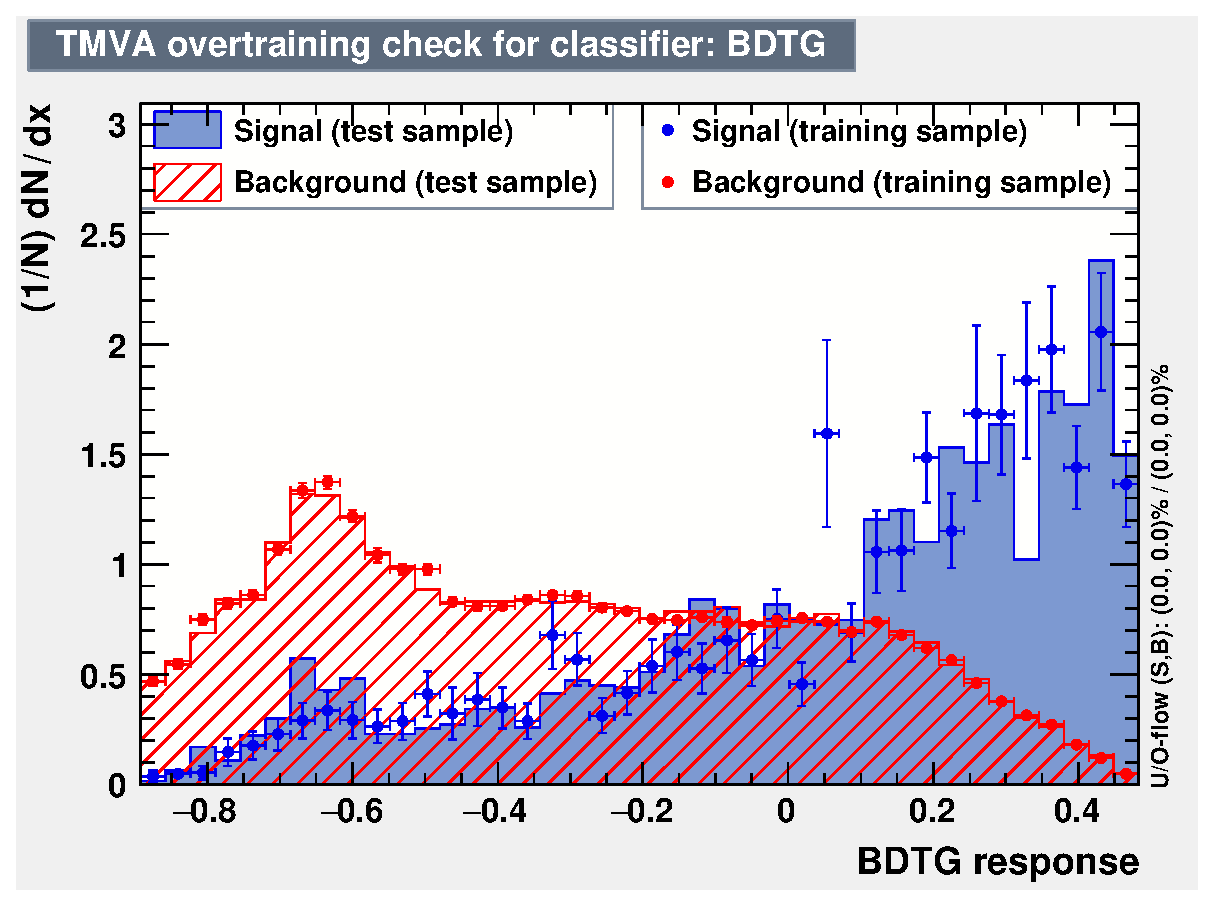
\includegraphics[width=0.4\linewidth]{Chapter5/overtrain_BDTG_merged.eps}
		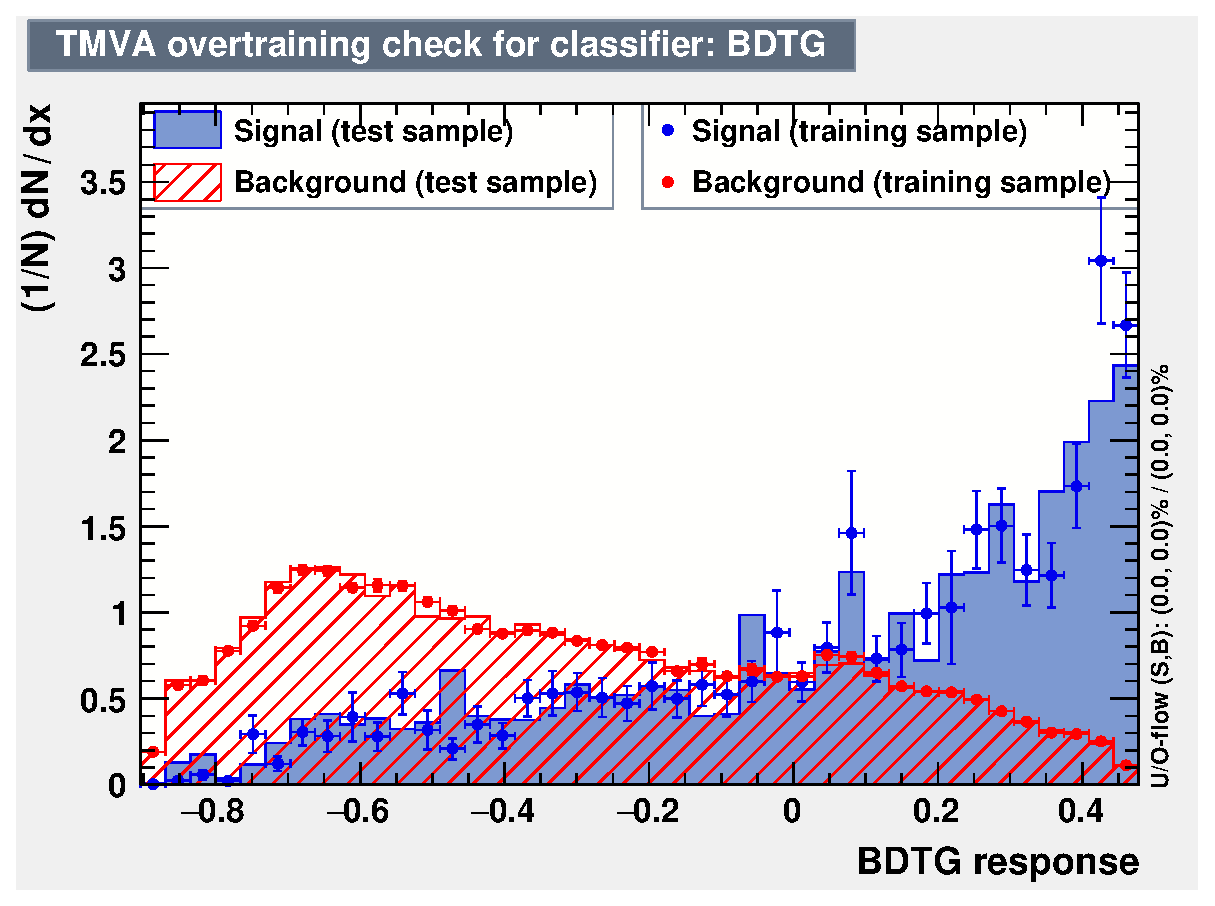
\includegraphics[width=0.4\linewidth]{Chapter5/overtrain_BDTG_trainEven_merged.eps}\\
		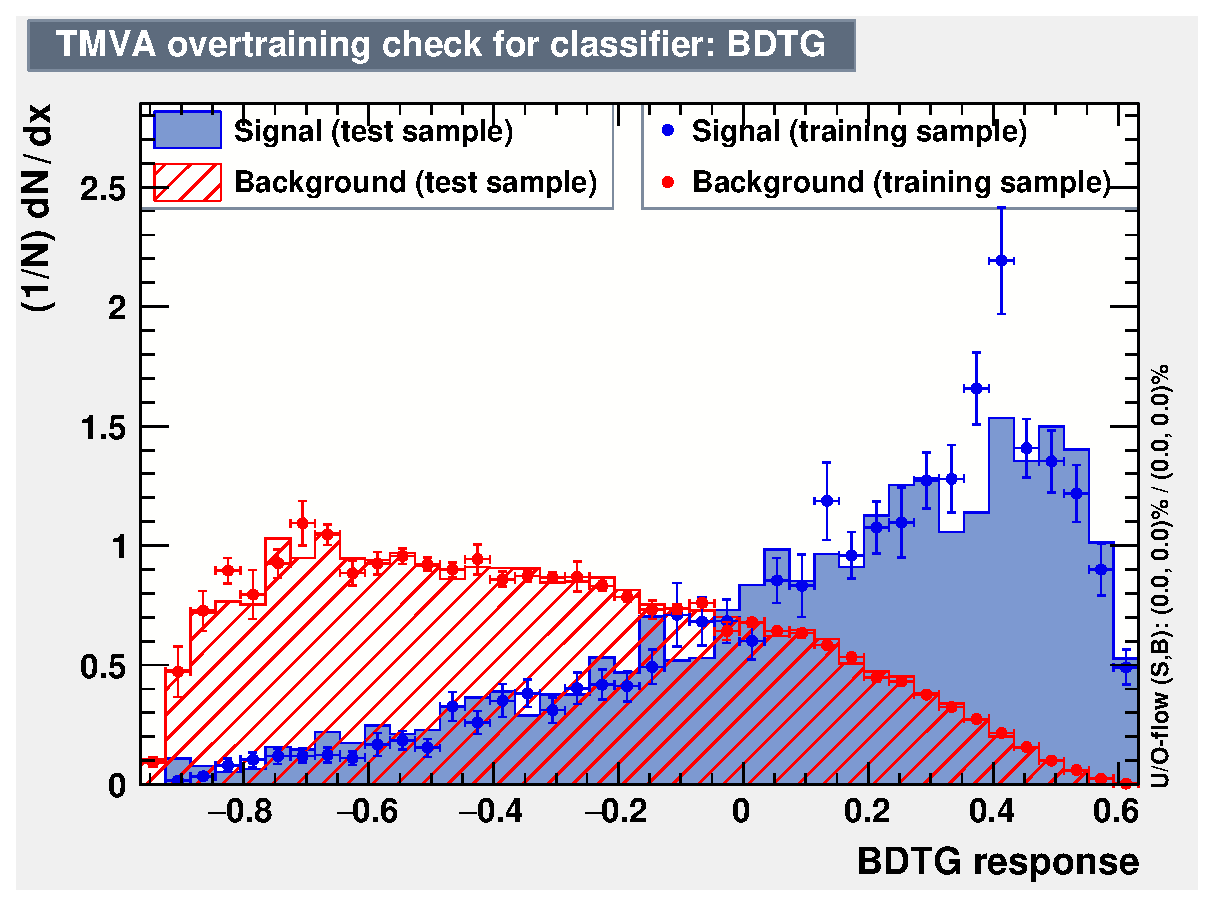
\includegraphics[width=0.4\linewidth]{Chapter5/overtrain_BDTG_resolved.eps}
		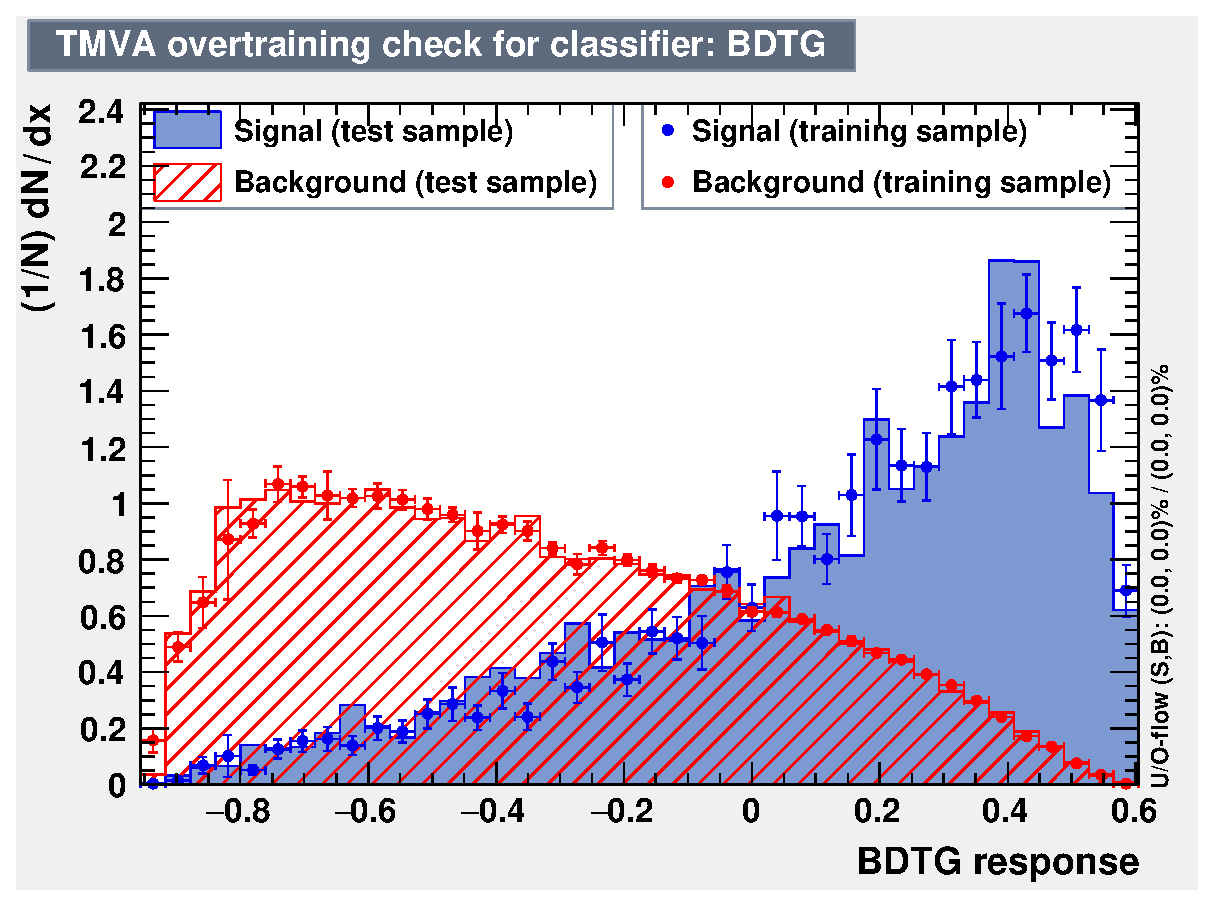
\includegraphics[width=0.4\linewidth]{Chapter5/overtrain_BDTG_trainEven_resolved.eps}
	\end{center}
	\caption[]{
		Comparison of test and training BDTG response distributions in 1-lepton channel, for merged (top) and resolved (bottom) regimes.
		Results obtained with even (odd) event numbers used for training are shown on left (right).
	}    
	\label{fig:BDT1lep}
\end{figure}
\section{Background Modeling}
The  modelling strategy is similar to the resonance search. The two dominant background interactions, $t\bar{t}$ and W+jets, are constrained using dedicated control regions, while the other subtle contributions are without constraint in the signal region fitting. However, to achieve higher precision measurement, some of the cuts are loosened. In this case, if the mismodelling of $m^{VBS}_{jj}$ is taken into the normalization fitting, it leads to huge uncertainty and degrade the sensitivity to measurement. Therefore, an extra event reweighting is applied on the W+jet MC events in the control region.
\\
\\The multijet background contribution in the non-resonance search is higher than the resonance analysis due to the lack of anti-QCD cuts from the topological variables. It is also estimated with the same fake factor from resonance search, because the distribution shape is supposed to remain the same with similar final state. The comparison between data and background (pre-fit) will be presented in next section along with the post-fit distribution. 
\subsection{VBS $m_{jj}$ Modelling}
As what was observed in the resonance search, an unknown issue is underlying in the simulation for W+jet events with Sherpa. With the comparison to data, a slope could be seen on the ratio of data to simulation in $m_{jj}^{VBS}$ distribution shown in Fig.~\ref{Fig:mtagmis}, and Madgraph sample gives better agreement. However, Sherpa sample has more events for statistics, so it is chosen for the estimation on W+jets background. 
\begin{figure}
	\begin{center}
		\includegraphics[width=0.6\linewidth]{Chapter5/boosted_mjj_tag.pdf}
	\end{center}
	\caption[]{
		Comparison of data and W+jets MC samples from Sherpa and Madgraph 5 in the boosted W+jets control region.
	}    
	\label{Fig:mtagmis}
\end{figure}
\noindent
To remodel the distribution, an extra weight is derived with $m_{jj(J)}^{VBF}$ distribution in W+jets control region:
\begin{equation}
w(m^{VBS}_{jj}) = \frac{N^{data}-(N^{mc}-N^{mc( W+jets)})}{N^{mc( W+jets)}} 
\end{equation}  
The estimation is performed as a linear fitting in $m_{jj(J)}^{V}$ bins:
\begin{equation}
m_{jj(J)}^{V} = [50,60,70,100,150,200,300] [GeV]
\end{equation}  
where the bin of 70-100 GeV is removed because it is defined as signal region. The fitting in multiple bins is to investigate the weight dependence on  $m_{jj(J)}^{V}$. The result of fitting could be seen in Fig. \ref{Fig:mjj_dataMC_fit_resolved} and \ref{Fig:mjj_dataMC_fit_boosted}. With consistent result between each $m_{jj(J)}^{V}$ slice, it was determined to single fitting function for the reweighting, and the parameters employed is shown in Tab~\ref{tab:reweighting_summary_Wjets} with $1\sigma$ uncertainty from statistical fluctuation. 
\begin{table}[!h]
	\caption{Estimated $m_{jj}^{VBS}$ reweighting functions for W+jets events.}
	\label{tab:reweighting_summary_Wjets}
	\centering
	\begin{tabular}{lccc}
		\hline
		Fitting parameters            & Resolved             & Merged   \\
		\hline
		$p_0$ (constant)              & $ 1.1 \pm 0.04 $       &  $ 1.1 \pm 0.02 $    \\
		$p_1$ (slope) [$GeV^{-1}$]    & $ -0.00021 \pm 0.00002 $ &  $ -0.00019 \pm 0.00003 $  \\
		\hline
	\end{tabular}
\end{table}
As the discrepancy was only seen in $m_{jj}^{VBS}$, the validation was performed by applying the weight in the other distributions, and the result is in Fig.~\ref{Fig:mjjtag_rwt_Wjets} which is showing the agreement is significantly improved for $m_{jj}^{VBS}$ distribution with little disturbance on the other kinematic properties.
\begin{figure}[ht]
	\centering
	\includegraphics[width=0.45\textwidth]{Chapter5/2para_msigJJ50to60.pdf}
	\includegraphics[width=0.45\textwidth]{Chapter5/2para_msigJJ60to70.pdf}
	\includegraphics[width=0.45\textwidth]{Chapter5/2para_msigJJ100to150.pdf}
	\includegraphics[width=0.45\textwidth]{Chapter5/2para_msigJJ150to200.pdf}
	\includegraphics[width=0.45\textwidth]{Chapter5/2para_msigJJ200to300.pdf}
	\caption{\label{Fig:mjj_dataMC_fit_resolved} Fit of $m^{VBS}_{jj}$ slope in W+jets resolved CRs, in different slices of $m^{V}_{jj}$. }
\end{figure}


\begin{figure}[!ht]
	\centering
	\includegraphics[width=0.45\textwidth]{Chapter5/2para_50to60.pdf}
	\includegraphics[width=0.45\textwidth]{Chapter5/2para_60to70.pdf}
	\includegraphics[width=0.45\textwidth]{Chapter5/2para_100to150.pdf}
	\includegraphics[width=0.45\textwidth]{Chapter5/2para_150to200.pdf}
	\includegraphics[width=0.45\textwidth]{Chapter5/2para_200to300.pdf}
	\caption{\label{Fig:mjj_dataMC_fit_boosted} Fit of $m^{VBS}_{jj}$ slope in W+jets boosted CRs, in different slices of $m^{V}_{J}$. }
\end{figure}

\begin{figure}[!ht]
	\centering
	\includegraphics[width=0.45\textwidth]{Chapter5/resolved_mjj_tag_sub.pdf}	\includegraphics[width=0.45\textwidth]{Chapter5/lvjjmass_sub.pdf}
	\includegraphics[width=0.45\textwidth]{Chapter5/boosted_mjj_tag_sub.pdf}
	\includegraphics[width=0.45\textwidth]{Chapter5/lvJmass_sub.pdf}
	\caption{\label{Fig:mjjtag_rwt_Wjets}
		Comparison of $m_{jj}^{VBS}$ and $m_{VV}$ distributions before and after the $m_{jj}^{VBS}$ reweighting for events in the resolved (top) and boosted (bottom) W+jets control regions 
	}
\end{figure}
\section{Statistical Interpretation}
The statistical interpretation of the non-resonance search follows the same strategy as the resonance one in likelihood construction (it has the same structure as Eq.~\ref{Eq. ML_all}), fitting, and then the final result. However, as the main focus of this analysis is to observe the vector boson scattering in the semileptonical ($qq\to VVjj \to \ell\ell qq/\ell\nu qq/\nu\nu qq +jj$), the exclusion interpretation is not performed. 
\\
\\The likelihood construction was using two discriminant: the BDT distribution for signal region (first line in Eq.~\ref{Eq. ML_all}) and the $m^{VBS}_{jj}$ for W+jet control region (third line in Eq.~\ref{Eq. ML_all}). The top control region was just taking one bin for the fitting normalization (second line in Eq.~\ref{Eq. ML_all}) which has summed over both $t\bar{t}$ and single top backgrounds. They are summarized in Tab.~\ref{tab:fitregions_1lep}. This choice is to make the $m^{VBS}_{jj}$ reweighting systematic uncertainty constrained by $m^{VBS}_{jj}$ distribution shape in the W+jet control region. 
\begin{table}[htb!]
	\centering
	\begin{tabular}{lccc}
		\toprule\midrule
		\multirow{2}{*}{Regions} & \multicolumn{3}{c}{1lep channel fit model} \\
		\cmidrule{2-4}
		& Merged high-purity & Merged low-purity & Resolved \\
		\midrule
		%SR     & \checkmark & \checkmark & \checkmark \\
		%WCR    & \checkmark & \checkmark & \checkmark \\
		SR     & BDT & BDT & BDT \\
		WCR    & $m^{VBS}_{jj}$& $m^{VBS}_{jj}$ & $m^{VBS}_{jj}$ \\
		%TopCR  & \checkmark & \checkmark & \checkmark \\
		TopCR  & One bin & One bin & One bin \\
		\midrule
		\bottomrule
	\end{tabular}
	\caption{\label{tab:fitregions_1lep} Summary of the regions from 1lep channel entering the likelihood of the fit models. 
		``One bin'' implies that a single bin without any shape information is used in the corresponding fit region.}
\end{table}

For the systematic uncertainties, the set from the resonance search is also applied. However, as the analysis employs the $m^{VBS}_{jj}$ reweight, the additional systematic uncertainty is taken in for the statistic uncertainty from this sources. The other addition systematic uncertainty arises from the interference between the QCD interactions and the VBS process, and it is taken into the uncertainty of signal modelling. 

\subsection{Fitting}
The fitting procedure is conducted as the resonance search for which the two dominant backgrounds, W+jets and top, are constrained by the dedicated control regions by a Gaussian distribution. Before having the final result of the signal strength, the background only fitting is performed to test the background modelling and the nuisance parameter effect on the fitting quality.
\\
\\{\bf Post-fit and Pre-fit Distributions} 
\\
\\The background and data comparison is presented here to verify the background modelling before the fitting. The post-fit plots are presented together to show the effect of fitting on the histograms. This fitting procedure has applied the background only hypothesis ($\mu=0$).
\\
\\Fig.~\ref{Fig:data_mc_vbs_wcr} and \ref{Fig:data_mc_vbs_tcr} are the results in w+jet and top control regions respectively. 
\begin{figure}[!ht]
	\centering
	\includegraphics[width=0.42\textwidth]{Chapter5/BDT_1lep_HP_WCR_prefit.pdf}	\includegraphics[width=0.42\textwidth]{Chapter5/BDT_1lep_HP_WCR_postfit.pdf}
	\includegraphics[width=0.42\textwidth]{Chapter5/BDT_1lep_LP_WCR_prefit.pdf}
	\includegraphics[width=0.42\textwidth]{Chapter5/BDT_1lep_LP_WCR_postfit.pdf}
	\includegraphics[width=0.42\textwidth]{Chapter5/BDT_1lep_res_WCR_prefit.pdf}
    \includegraphics[width=0.42\textwidth]{Chapter5/BDT_1lep_res_WCR_postfit.pdf}	
	\caption{\label{Fig:data_mc_vbs_wcr}
		Comparison of the BDT score distributions before and after the fitting in the  
		Boosted HP (top), Boosted LP (middle), resolved (bottom) W+jet control regions. The left and right are the plots for pre-fit and post-fit (with the post-fit over pre-fit ratio) results. 
	}
\end{figure}
\begin{figure}[!ht]
	\centering
	\includegraphics[width=0.42\textwidth]{Chapter5/BDT_1lep_HP_CRTop_prefit.pdf}	\includegraphics[width=0.42\textwidth]{Chapter5/BDT_1lep_HP_CRTop_postfit.pdf}
	\includegraphics[width=0.42\textwidth]{Chapter5/BDT_1lep_LP_CRTop_prefit.pdf}
	\includegraphics[width=0.42\textwidth]{Chapter5/BDT_1lep_LP_CRTop_postfit.pdf}
	\includegraphics[width=0.42\textwidth]{Chapter5/BDT_1lep_res_CRTop_prefit.pdf}
	\includegraphics[width=0.42\textwidth]{Chapter5/BDT_1lep_res_CRTop_postfit.pdf}	
	\caption{\label{Fig:data_mc_vbs_tcr}
             Comparison of the BDT score distributions before and after the fitting in the  
             Boosted HP (top), Boosted LP (middle), resolved (bottom) top control regions. The left and right are the plots for pre-fit and post-fit (with the post-fit over pre-fit ratio) results. 
	}
\end{figure}
\noindent
\\
\\{\bf Fitting Quality}
\\
\\The fitting quality is also verified in this analysis with the pulls and the correlation matrix. The combined results of merged and resolved channels are in Fig.~\ref{Fig:fit_quality} with a reduced scheme presenting only the NPs with significant correlation or pulls on the fitting. There are a coupling of NPs like $m^{VBS}_{jj}$ reweighting which are highly constrained and pulled, and that is due to the strong impact of the systematic uncertainties on the distribution shape. 
\begin{figure}[!ht]
	\centering
	\includegraphics[width=0.56\textwidth]{Chapter5/ranking_data_1lepCR.pdf}	
	\includegraphics[width=0.68\textwidth]{Chapter5/corr_data_1lepCR.pdf}	
	\caption{\label{Fig:fit_quality} The fitting quality is verified by the pulls(up) and variable correlation(bottom). They are in the reduced scheme to show off the notable ones.  
	}
\end{figure}

\subsection{Results}
This analysis is aiming to provide the vector boson scattering measurement which has been predicted by the SM, so the interpretation has the following two parts: a) the discovery significance b) the cross-section in the intended final states in the fiducial region, and the exclusion limit is not set. 
\\
\\{\bf Combination of Semileptonic Channels}
\\
\\For this analysis, all the three semi-leptonic channels are considered. The results will be showing the combination of all the three semileptonical channels through the combination procedurediscussed in the last chapter. Most of the systematic uncertainties are correlated among the three semileptonic final states ($\ell\ell qq$, $\ell\nu qq$, and $\nu\nu qq$), but the ones for normalization factors and the multijet background (only in the $\ell\nu qq$ channel) are taken decorrelated. The details of the other two channels could be referred to \cite{Aad:2019xxo}. In addition, the combination performed the simultaneous fitting on the three channels which means that the signal strength and the scaling factors among the three channels are shared: signal strength of three of them, W+jet and top scaling factor are shared between $\ell\nu qq$ and $\nu\nu qq$ which are constrained in $\ell\nu qq$ control regions, and Z+jet scaling factor is shared between $\ell\ell qq$ and $\nu\nu qq$ which is constrained in the $\ell\ell qq$ Z+jet control region. The yields after the fitting with the signal in the $\ell\nu qq$ channel are presented in Tab.~\ref{tab:yields_vbs} for the control and signal regions, and the scale factors on W+jets and top backgrounds are shown in Tab.~\ref{Tab:lvqq_fittedsf}.
\begin{table}[tbp]
	\renewcommand{\arraystretch}{1.25}
	\caption{Expected and observed yields in signal and control regions for the signal hypothesis.  Yields and uncertainties are evaluated after the fitting to the data in all $\ell\nu qq$ regions indicated above.}
	\centering
		\begin{adjustbox}{center}
		\resizebox{1.1\textwidth}{!}{%
			\begin{tabular}{| c | c@{\ $\pm$\ }c c@{\ $\pm$\ }c c@{\ $\pm$\ }c | c@{\ $\pm$\ }c  c@{\ $\pm$\ }c c@{\ $\pm$\ }c | c@{\ $\pm$\ }c  c@{\ $\pm$\ }c c@{\ $\pm$\ }c |}
				\hline
				\hline
				&\multicolumn{6}{c|}{Boosted, High Purity}  &\multicolumn{6}{c|}{Boosted, Low Purity}  &\multicolumn{6}{c|}{Resolved}   \\
				\cline{1-19}
				&\multicolumn{2}{c}{               SR}&\multicolumn{2}{c}{      $W$+jets CR}&\multicolumn{2}{c|}{           Top CR}&\multicolumn{2}{c}{    Signal Region}&\multicolumn{2}{c}{      $W$+jets CR}&\multicolumn{2}{c|}{           Top CR}&\multicolumn{2}{c}{               SR}&\multicolumn{2}{c}{      $W$+jets CR}&\multicolumn{2}{c|}{           Top CR}\\
				\hline
				$W$+jets    & 1556.66&244.61 & 1448.88&154.05 &  749.76&121.50  & 3931.65&539.85 & 2002.27&272.88 & 1822.72&244.59 & 97489.49&22840.18 & 25321.33&4730.05  &  35265.68&7019.05   \\
				Top         & 570.42&123.89 &  136.60&45.84 & 5635.05&1198.20 &  608.91&142.16 &  166.52&51.80 & 6670.66&1649.92 & 11747.76&3529.05 &  1277.32&634.75 & 128305.05&36872.78  \\
				SM Diboson  &  238.63&66.59  &  73.92&20.90  &   181.79&52.32  &   339.94&107.33 &  92.97&30.69 &   189.66&56.52  &  4330.69&1287.57  &   581.58&162.93  &  2093.22&560.53    \\
				$Z$+jets    &   53.47&9.96   &  40.73&6.95  &   28.42&0   &   123.62&20.22  &   57.37&11.74  &   72.81&14.09   &  3939.25&1667.54  &   954.46&350.69  &   1614.46&432.94    \\
				Multijet    &\multicolumn{2}{c}{--}&\multicolumn{2}{c}{--}&\multicolumn{2}{c|}{--}&\multicolumn{2}{c}{--}&\multicolumn{2}{c}{--}&\multicolumn{2}{c|}{--}& 
				15381.16&2292.91 & 3776.57&471.86 & 24426.45&4082.85 \\
				\hline
				Background&        2477.59&382.38 & 1705.67&186.99  & 6642.85&1268.24  & 5047.75&707.29 & 2325.75&320.31 & 8797.59&1784.29 & 133347.69&26918.73  & 31959.56&5264.22  & 192183.01&40519.71   \\
				\hline
				VBS Signal&        58.41&8.32  & 5.53&0.97 & 47.84&7.76 & 43.62&6.05 & 6.53&1.43 &41.75&6.24 & 459.33&54.23 & 48.30&4.89 & 478.14&65.29 \\
				\hline
				SM Total  &      2536.00&382.47 & 1711.20&186.99 & 6690.69&1268.26 & 5091.37&707.32 & 2332.28&320.31 & 8839.34&1784.30 & 133807.02&26918.78 & 32007.86&5264.22 & 192661.15&40519.76 \\
				\hline
				Observed&\multicolumn{2}{c}{1929}      &\multicolumn{2}{c}{1364}             &\multicolumn{2}{c|}{5806}             &\multicolumn{2}{c}{3709}              &\multicolumn{2}{c}{1831}             &\multicolumn{2}{c|}{7629}             &\multicolumn{2}{c}{104476}            &\multicolumn{2}{c}{27475}             &\multicolumn{2}{c|}{157177}             \\
				\hline
				\hline
			\end{tabular}
		}
		\label{tab:yields_vbs}
	\end{adjustbox}
\end{table}
\begin{table}
	\begin{center}
			\begin{tabular}{|l|c|c|c|}
				\hline
				channel & resolved & merged \\
				\hline
				W+jet CR & $0.93\pm0.07$ & $0.86\pm0.06$ \\
				\hline
				Top CR &   $0.67\pm0.10$ & $0.83\pm0.01$ \\
                \hline
			\end{tabular}

		\caption{The scale factors for the top and W+jet backgrounds for the fitting with signal}
		\label{Tab:lvqq_fittedsf}
	\end{center}
\end{table}
\noindent
\\
\\{\bf Discovery Significance}
\\
\\The asymptotic formulae is applied here with the same methodology from the resonance search to test the SM VBS hypothesis against the null hypothesis. The discovery significance with the test statistics in Eq.~\ref{Eq:Sig_testQ} before the batman veto is shown in Tab.~\ref{tab:significance_sbfit_obs} for each channel and combination. However, with the event removal from this cut, the final discovery significance was given just 2.7. Fig.~\ref{fig:fit_mu_VBS_obs} is showing the signal strengths denoted, $\hat{\mu}$, giving the best fit in each individual channel and the combination. The signal and background distributions with observed data are re-binned into the $\log(S/B)$ and presented in Fig.~\ref{fig:SoBplot_obs}. The final combined result has great agreement with the SM prediction, and the sensitivity is dominated by the systematic uncertainty. The compatibility of the three channels are within the $36\%$ with the estimation from the $\chi^2$ distribution of two degrees of freedom (from systematic and statistical uncertainties). 
\begin{table}[htb] 
	\centering
	\begin{tabular}{ccc}
		\hline
		Channel  & Exp. significance(Asimov) & Obs. significance  \\ 
		\hline
		$\nu\nu qq$ & 1.35 & 1.43 \\
		$\ell\nu qq$ & 1.77 & 0.53 \\
		$\ell\ell qq$ & 1.34 & 2.07 \\
		combined & 2.58  & 3.14 \\
		\hline 
	\end{tabular}
	\caption{Summary of VBS signal significance against null-hypothesis in the semileptonic final states.}
	\label{tab:significance_sbfit_obs}  
\end{table}
\begin{figure}[!h]
	\begin{centering}
		\includegraphics[width=10cm]{Chapter5/Muhat_VBS_channels_obs.pdf} 
		\caption{$\hat{\mu}$ for each individual channel and combined.}
		\label{fig:fit_mu_VBS_obs}  
	\end{centering}
\end{figure}
\begin{figure}[!h]
	\begin{centering}
		\includegraphics[width=10cm]{Chapter5/Global_SoverB_2016.pdf} 
		\caption{Event yields as a function of $log_{10}(S/B)$. Final-discriminant bins in all regions are combined into bins of
			$log_{10}(S/B)$, with the expected signal, $S$ and background $B$.}
		\label{fig:SoBplot_obs}  
	\end{centering}
\end{figure}
\\
\\{\bf VBS Cross-Section Measurement}
\\
\\To measure the inclusive cross-section of the VBS production, the selection efficiency is estimated with the generator truth information through an approach like the tag-and-probe method. Firstly, the events from signal simulation are tagged via the ``fiducial region'' selection, which means the same signal region cuts are applied on events at the particle truth (``truth'') level (without considering their interactions with the detector), but the D2 cuts are removed, as it is a variable at the reconstruction level. Then, those tagged events are probed by whether the reconstructed particles (``reco'') could also pass the same cuts. This would then give the reconstruction efficiency:
\begin{equation}
\mathcal{C}_{eff} = \frac{N(reco)}{N(truth)} 
\end{equation}  
To measure the cross-section, the signal strength is set as a free parameter, and the related uncertainty should not affect the fitting procedure, so it is removed from the likelihood reconstruction in Eq.~\ref{Eq. ML_all}. Then, the cross-section could be presented as:
\begin{equation}
\sigma\times BR=\frac{\mu\times (N^{data}-N^{bkg})}{\mathcal{C}_{eff}\times\mathcal{L}}
\end{equation}
The result of the cross-section measurement could be seen in Tab.~\ref{tab:obs_mu_fidxs}.
\begin{table}[htb] 
	\centering
	\begin{tabular}{lcc}
		\hline
		Fiducial region  & Predicted $\sigma_{exp} $  & Measured $\sigma_{exp}$ \\
		\hline
		Total    & $43.0 \pm 2.4 $ (theo.)~fb  &  $45.1 \pm 8.6$ (stat.) $~^{+15.9}_{-14.6}$ (sys.)~fb \\
		Merged   & $11.4  \pm 0.7 $ (theo.)~fb  & $12.7 \pm 3.8$ (stat.) $~^{+4.8}_{-4.2}$ (sys.)~fb \\
		Resolved & $31.6 \pm 1.8 $ (theo.)~fb  &  $26.5 \pm 8.2$ (stat.) $~^{+17.4}_{-17.1}$ (sys.)~fb \\
		\hline 
	\end{tabular}
	\caption{Summary of measured signal strengths, and the predicted and measured fiducial cross section.
	}
	\label{tab:obs_mu_fidxs}  
\end{table}
\section{Summary}
This analysis is dedicated to spot the vector boson scattering interaction in the semileptonical final states with the analysis strategy inherited from the resonance search. The combination of the three final states ($\ell\ell qq$+$\ell\nu qq$+$\nu\nu qq$) has presented the discovery significance of $2.7\sigma$  against the null hypothesis, which is still not yet confident but still within reasonable agreement to the SM estimation ($2.5\sigma$). For the cross-section measurement, it was given $45.1~fb$ for the VBS process in agreement with the SM prediction within the uncertainties, and this is also the measurement of vector boson scattering in semileptonical final states. 